\documentclass[12pt]{article}

\usepackage{epsfig}
\usepackage{rotating}
\usepackage{lscape}
\usepackage{amsfonts}
\usepackage{amssymb}
\usepackage{theorem}
\usepackage{amsmath}
\usepackage{graphicx}
\usepackage{citesort}
\usepackage{float}
\usepackage{color}
\usepackage{array}
\usepackage{color}
\usepackage{array}
\usepackage{float}
\usepackage{url}
\usepackage{setspace}
%\usepackage{amsmath,amsfonts,amssymb,cite,array,graphicx}

\textwidth=17.36cm
\textheight=23.90cm
\hoffset=-2.37cm
\voffset=-2.5cm
\parskip=1pt

\renewcommand{\rmdefault}{ptm}

\newtheorem{definition}{Definition}[section]
\newtheorem{theorem}{Theorem}[section]
\newtheorem{corollary}{Corollary}[section]
\newtheorem{lemma}{Lemma}[section]
\newtheorem{remark}{Remark}[section]


\date{\small\today} \title{IAM851 Final Project} \author{Jeffrey Picard} 
\doublespacing

\begin{document}

\maketitle


\begin{abstract}
The purpose of this project is to gain experience with Fast Fourier Transforms (FFTs) and a commonly used FFT library called fftw by implementing an FFT
algorithm in C, in one and two dimensions, and comparing its performance to that of the existing library. Additionally this project gives an opportunity 
to use MPI by parallelizing the 2d FFT.
\end{abstract}


% main text
\section{Building and Using the Code}
The code for the project is packaged into a gzipped tarball (.tar.gz) with the use of 'make dist'. In order to build and run the code the first step
is to unpack it with 'tar xfzv' then 'cd' into the directory and run 'autoconf -i', followed by 'configure' and then 'make' to actually build the code.
Once this is done there will be multiple executables, many used for testing the various functions that were written in the course of completing this 
project. 

The ``mpi\_alltoall\_transpose\_test'' program tests doing a matrix transpose across processes with the ``MPI\_Alltoall'' function call. Currently
this test program requires on the number of processes used be equal to $\sqrt{N}$, $N$ the number of columns in an $N by N$ matrix. The actual 
parallelized FFT does not have this stipulation.

The ``fft\_jp\_mpi\_test'' program is the original test program used in writing the parallel 2d FFT algorithm and isn't used for anything beyond that.

The ``fftw\_test'' and ``fftw\_2d\_test'' programs use the fftw3 library to perform one and two dimensional FFTs respectively. These were the programs
used in to verify the results of the fft functions implemented for this project.

The ``fft\_jp\_test'' and ``fft\_jp\_2d\_test'' programs demonstrate how to use the code written for this project to actually perform the FFTs and
get the results. They were used to test the correctness of the fft algorithms. The ``fft\_jp\_2d\_test'' program is used to test the two different
flavors of the 2d fft function (explained in full later). When run with zero arguments it runs the first version which just outputs the result to 
a file. When run with any number of arguments it instead runs a version which returns the result of the computed fft in another argument passed to the
function.

The ``fft\_jp\_timing'' and ``fftw\_timing'' programs each take an integer argument for the number of tests that should be performed. As the
fft algorithms written for this project can only handle ffts of sizes that are powers of two, the tests will start at $2^1 = 2$ points, then $2^2=4$ points, etc
until they have all been performed. They will then output the results of the timing in a file. Figure \ref{1d_time} was created from this data.

The actual main use of the code written for this assignment is more as a few library functions rather than a program which solves a specific problem.
The rest of this document shall endeavor to explain the use of these functions, how they were implemented and compare their performance in terms
of the fftw library and how the parallel algorithm scales with more processors.

%\section{Output and Plots}

\begin{figure}
\begin{center}
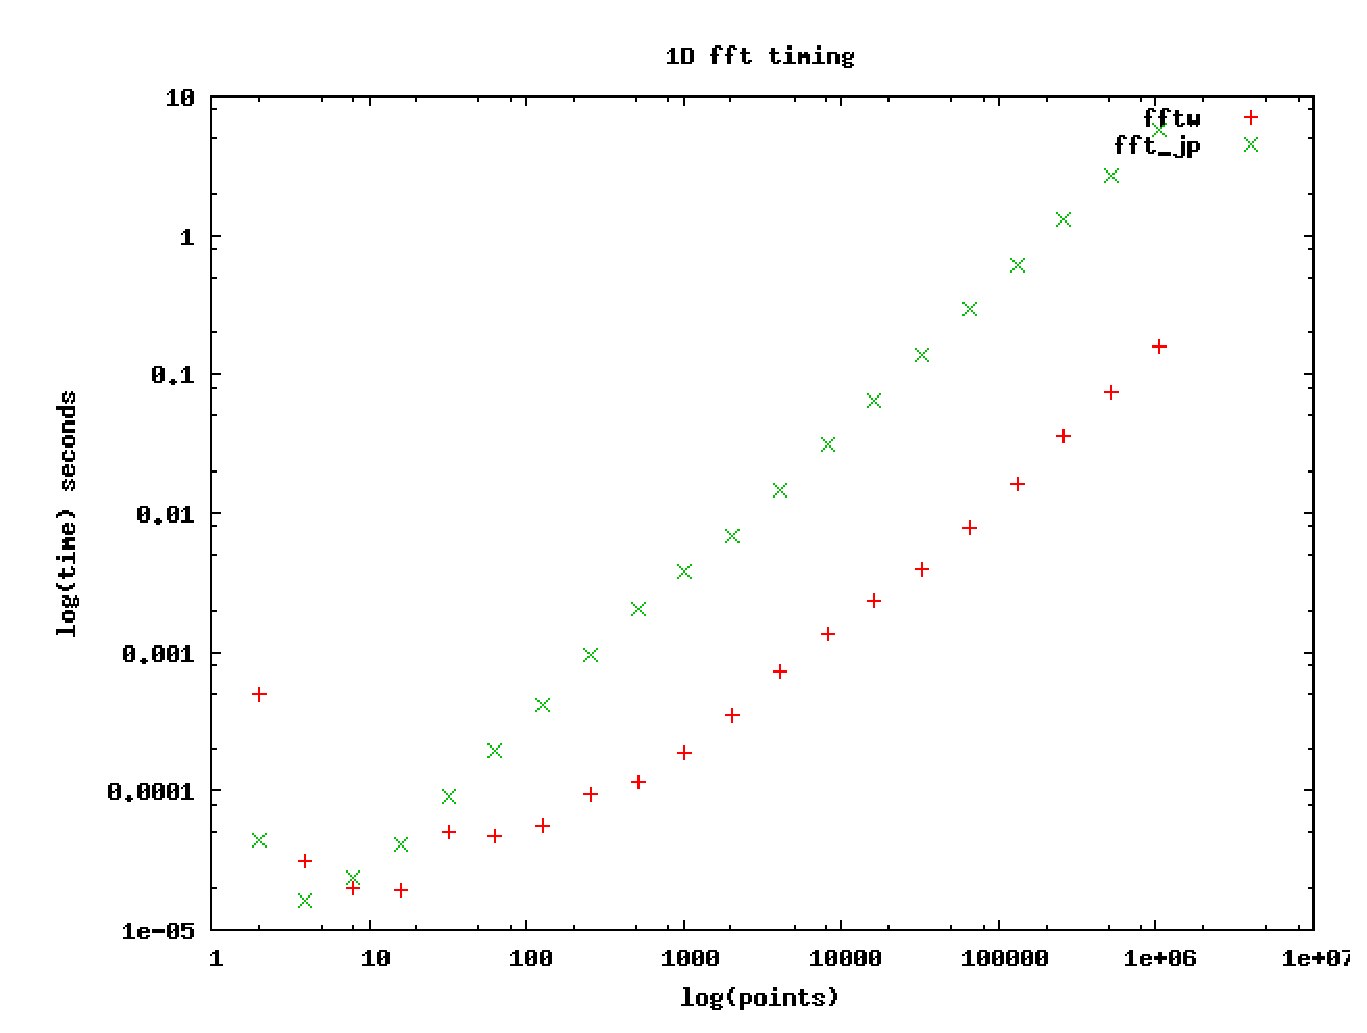
\includegraphics[scale=0.5]{figures/1d_timing.eps} \small \caption{Plot of timing for the 1d fft functions.\label{1d_time}}
\end{center}
\end{figure}

\begin{figure}
\begin{center}
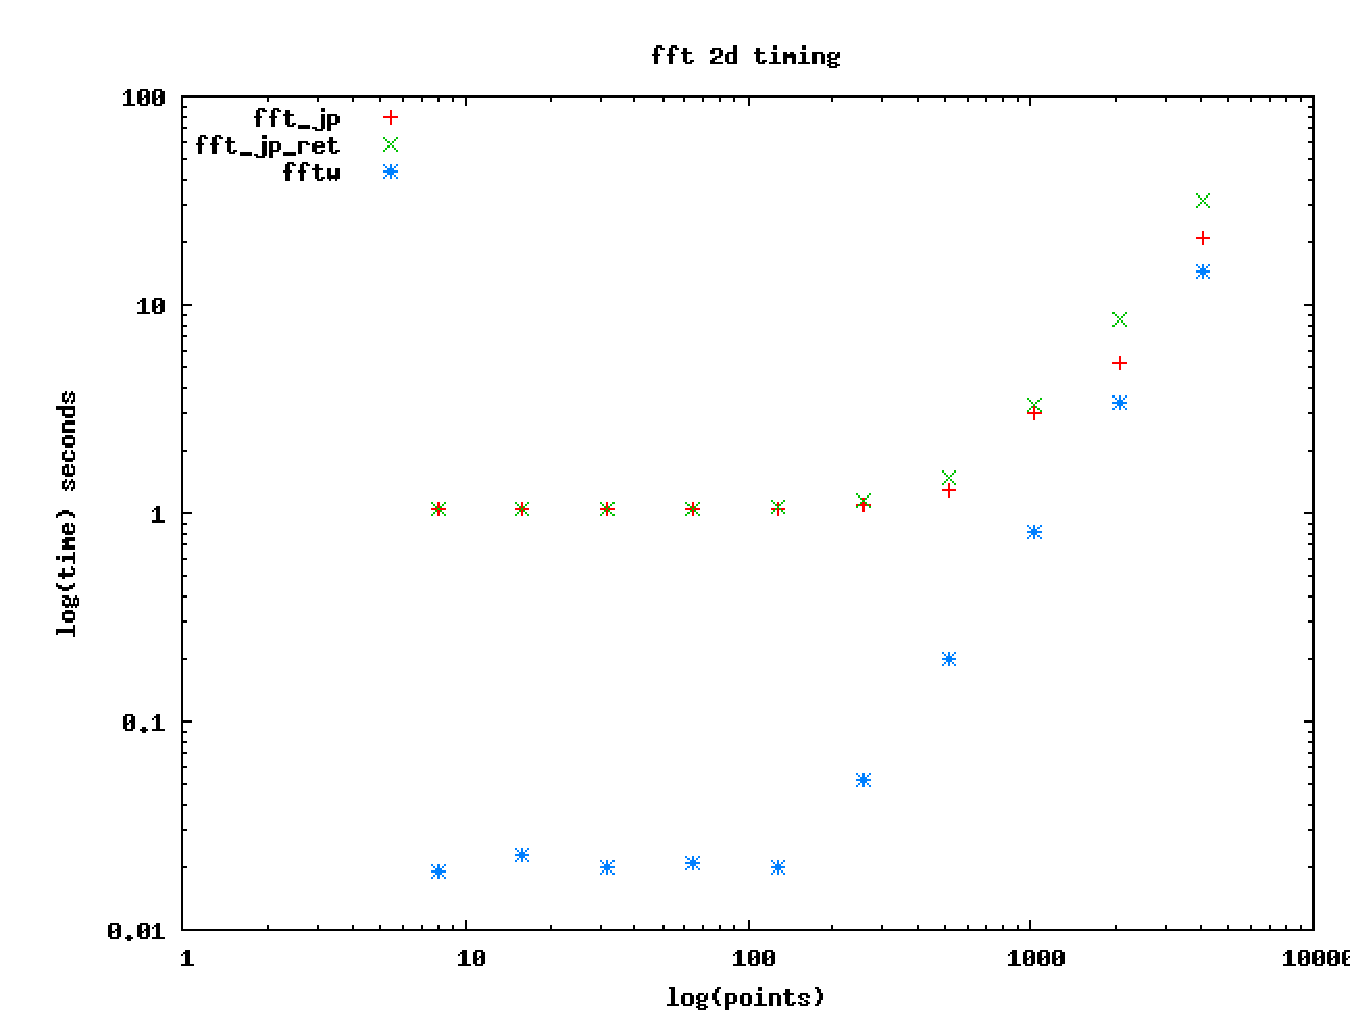
\includegraphics[scale=0.5]{figures/2d_timing.eps} \small \caption{Plot of timing for the 2d fft functions.\label{2d_time}}
\end{center}
\end{figure}

\begin{figure}
\begin{center}
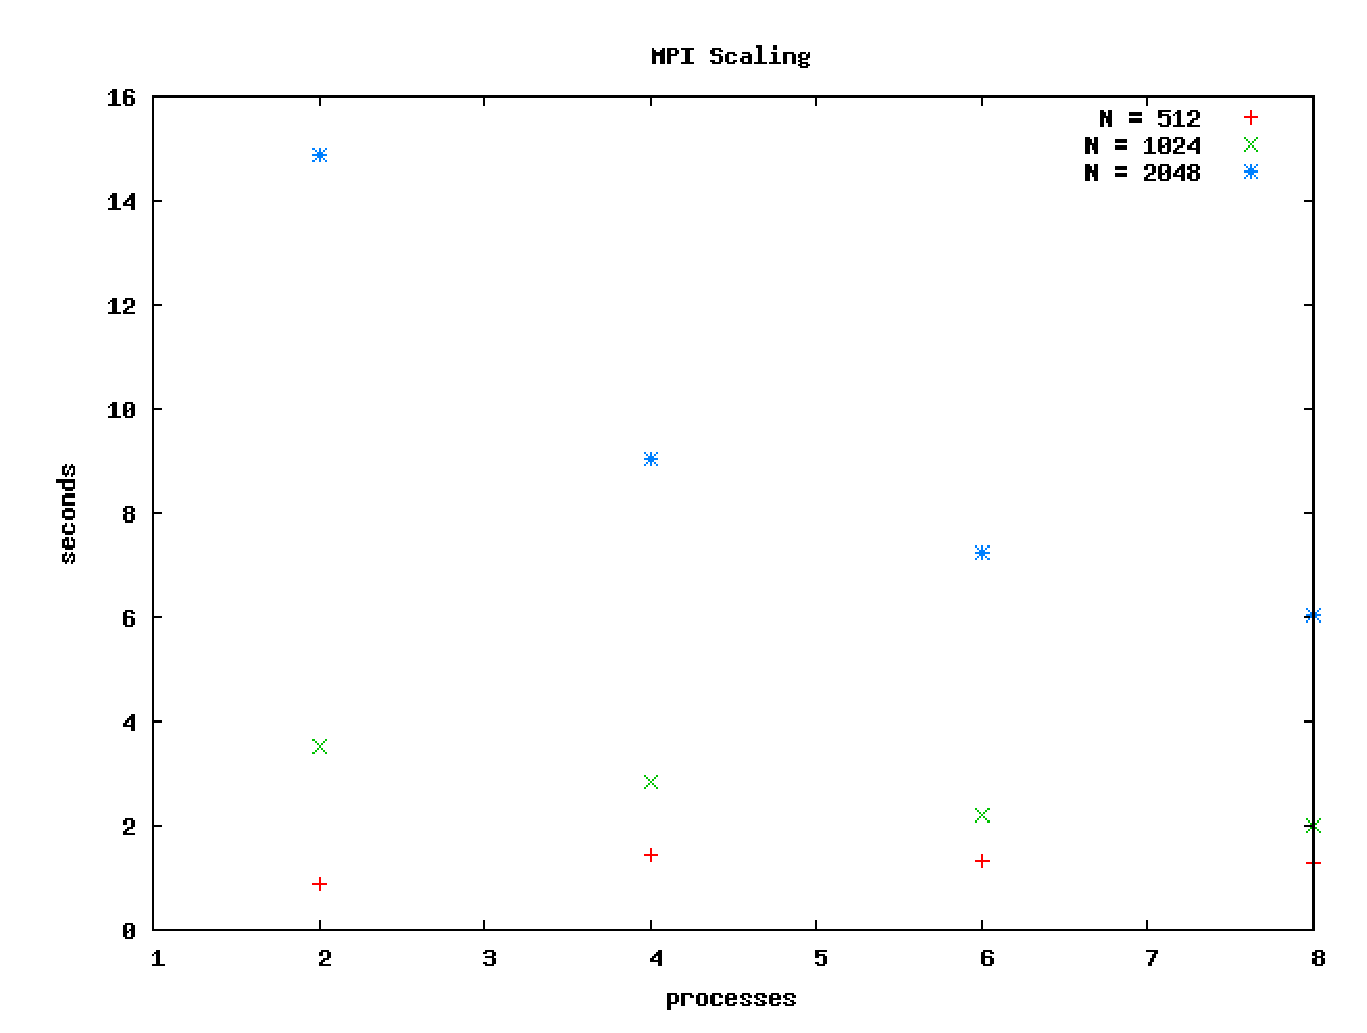
\includegraphics[scale=0.5]{figures/mpi_scaling.eps} \small \caption{Plot of MPI scaling showing time versus number of processes for N = 512, 1024 and 2048 point ffts.\label{scaling}}
\end{center}
\end{figure}


\section{Scaling with MPI}
As seen in Figure \ref{scaling} the parallel 2d fft using MPI doesn't scale well until
the number of points is above 512 (note the red points). Once that threshold is reached the scaling
is quite evident as seen in Figure \ref{scaling} (note the blue and green points) which show the 2d algorithm
being run on 1024 and 2048 points. Note that the number of points must
be a power of 2 and the number of processes must be a multiple of 2.

%\newpage

\section{Implementation}
The 1d FFT was implemented in a straight forward recursive method following
the pseudo code from lecture note slide 13 from \cite{Heath2011}. There are 
ways of implementing this iteratively
that are more efficient. i.e. using the binary reversal seen in FFTs, and
would probably have been more competitive with the fftw implementation.
However this method seemed much cleaner and served the purposes of this
project perfectly. This function is implemented as ``fft'' and is included
in the ``fft\_jp.h'' file. It takes an input vector, output vector and
a number of points. These vectors are the vector structs from class. There
is also an implementation called ``fft\_mpi'' which uses complex double
pointers instead of the vector struct because the 2d FFT was implemented with
complex double pointers instead of the struct.

In order to parallelize the 2d FFT the ``hyper cube'' approach was taken. Following this methodology each process is responsible for $c = N / p$ columns of
an $N$x$N$, matrix where $p$ is the number of processes. Each process then performs $c$, $N$-point 1d FFT's in serial (one for each column it is responsible for).
There is then a communication phase which uses ``MPI\_Alltoall'' in order to perform a matrix transpose across the processes. This part is fairly simple if
there are $N$ process running, so that each process is only responsible for one column. However as this is very often not the case (unless you have an arbitrary
large number of cores to distribute threads to as your data size grows) this becomes slightly more complicated. Another set of $c$, $N$-point 1d ffts are then
performed before finally re-transposing the matrix with ``MPI\_Alltoall'' once 
again and having the finished product. 

At least each process has their columns
of the matrix in a finished product form. In order to actually get this all
to a single array, like the one which the fftw\_2d function stores its
output in, another round of communication to a single process is required.
Doing this however takes significant time. See Figure \ref{2d_time} and note
that it is on a log scale. 

For this reason two different versions of this
function were implemented. ``fft\_2d'' takes a number of points and an input
array and then outputs the 2d fft result to files, one per process, instead
of communicating the result back to a single process. One point that needs
nothing here is that unlike the ``fftw\_2d'' which is more flexible, this
function only does $N$x$N$ 2d ffts. The size of the input vector it takes
is only $N$ and this same data is used for all of the columns.

The second version of this function is called ``fft\_2d\_ret'' and takes in
addition to the $N$-point input array, an $N$x$N$-point output array for 
the result, which is stored on the process with rank 0. As noted above and 
seen in Figure \ref{2d_time} this version
is slower due to the extra communication that is needed to get all the
information to one process.

\section{Conclusion}
In conclusion the speed of the 2d FFT showed significant speed improvement when parallelized, although not until large enough (greater than 512 points) data
sets were used. In the end though the serial versions of fftw still displayed performance which dominated that of any of the hand written FFT algorithms.
Further extensions of this work would be to remove the inflexibility of the
2d fft so that the full $N$x$M$ matrix may be specified as input data
and so that $N$ need not equal $M$. Also improved methods of performing
the 1d fft, such as with bit reversals, would be worth looking into.

\bibliographystyle{elsarticle-num}
\bibliography{fft}

\end{document}
